\nonstopmode

\documentclass[letterpaper,11pt,titlepage]{article}
\usepackage{amsthm,amssymb,mathtools}
\mathtoolsset{showonlyrefs}
\usepackage{bm}
\usepackage[margin=1in]{geometry}
\usepackage{booktabs}
\usepackage{enumitem}
\usepackage{framed}
\usepackage{tikz}
\usetikzlibrary{shapes,arrows,positioning,patterns,calc}
\usepackage{pgfplots}
\pgfplotsset{compat=1.9}
\usepackage{listings}
\usepackage[numbered,framed]{mcode}

\usepackage{algpseudocode}
\usepackage{algorithm}

\usepackage{fancyhdr}
\pagestyle{fancy}
\fancyhead{}
\fancyfoot{}
\fancyfoot[L]{K.\ Okkelberg}
\fancyfoot[R]{\thepage}
\renewcommand{\headrulewidth}{0pt}
\renewcommand{\footrulewidth}{0.5pt}

\newcommand*\dif{\mathop{}\!\mathrm{d}}
\newcommand{\trans}{^\text{T}}
\newcommand{\herm}{^\text{H}}
\DeclareMathOperator{\E}{E}
\DeclareMathOperator{\trace}{trace}
\DeclareMathOperator{\sign}{sign}
\let\Pr\relax
\DeclareMathOperator{\Pr}{P}
\newcommand*\pder[2]{\frac{\partial #1}{\partial #2}}
\newcommand*\R{\mathbb{R}}

\tikzstyle{line} = [draw,>=latex]
\tikzstyle{dot} = [circle,fill=black,inner sep=0pt,minimum size=4pt]

\begin{document}

\title{ECE 6553: Homework \#3}
\author{Klaus Okkelberg}
\date{March 14, 2017}
\maketitle

\setlist{listparindent=\parindent}

\begin{enumerate}[leftmargin=0pt]

\item Let the Lagrange multiplier for this new problem be $\mu(t)=[\mu_x\trans(t)\ \mu_\lambda\trans(t)]\trans$. Then, the Hamiltonian is $H = \mu\trans F$.

  The optimal $\lambda_0$ that solves the Bolza problem results in $\mu_\lambda(0)=0$, where $\mu(t)$ satisfies
  \begin{align}
    \dot\mu &= -\pder{H\trans}{z} = -\pder{}{z}
              \begin{bmatrix}
                \dot x & \dot\lambda
              \end{bmatrix} \begin{bmatrix}
                \mu_x \\ \mu_\lambda
              \end{bmatrix} \\
            &= -\pder{}{z} \left\{
              f\trans(x,u^*(x,\lambda))\mu_x - \pder{H\trans(x,u^*(x,\lambda),\lambda)}{x} \mu_\lambda
              \right\} \\
            &= \begin{bmatrix}
              \displaystyle -\pder{f\trans}{x}\mu_x + \pder{}{x} \pder{H\trans}{x} \mu_\lambda \\[2ex]
              \displaystyle -\pder{f\trans}{\lambda}\mu_x + \pder{}{\lambda} \pder{H\trans}{x}\mu_\lambda
            \end{bmatrix} \\
    \mu(T) &= \pder{C(z(T))}{z} = \pder{}{z} \left\Vert \lambda(T) - \pder{\Psi(x(T))}{x} \right\Vert^2 \\
            &= \begin{bmatrix}
              \displaystyle -2 \left(\lambda(T) - \pder{\Psi(x(T))}{x}\right)\trans \pder{^2 \Psi(x(T))}{x^2} \\[2ex]
              \displaystyle 2 \left(\lambda(T) - \pder{\Psi(x(T))}{x}\right)
            \end{bmatrix}
  \end{align}
  For given $\gamma,\varepsilon>0$, the algorithm that finds the optimal $\lambda_0$ is given by

  \begin{algorithm}
    \begin{algorithmic}
      \State Pick $\lambda_0$
      \State $z(0) \coloneqq \begin{bmatrix}
        x_0 \\ \lambda_0
      \end{bmatrix}$
      \Repeat
      \State Simulate $z(t)$ from $z(0)$ over $[0,T]$
      \State Simulate $\mu(t)$ backwards from $\mu(T)$ using $z(t)$
      \State Update $\lambda_0 \coloneqq \lambda_0 - \gamma \mu_\lambda(0)$
      \State Update $z(0) \coloneqq \begin{bmatrix}
        x_0 \\ \lambda_0
      \end{bmatrix}$
      \Until $\Vert \mu_\lambda(0) \Vert \le \varepsilon$
    \end{algorithmic}           
  \end{algorithm}

\item \begin{enumerate}
  \item 
    \begin{align}
      H &= \frac12 (u_1^2 + u_2^2) + \lambda_1 u_1 + \lambda_2 u_2 + \lambda_3 (x_1u_2 - x_2u_1) \\
      \pder{H}{u_1} &= u_1 + \lambda_1 - \lambda_3 x_2 = 0 \\
      \pder{H}{u_2} &= u_2 + \lambda_2 + \lambda_3 x_1 = 0 \\
      \Longrightarrow \Aboxed{u^* &= \begin{bmatrix}
          -\lambda_1 + \lambda_3 x_2 \\
          -\lambda_2 - \lambda_3 x_1
        \end{bmatrix}} \\
      \dot\lambda &= -\pder{H\trans}{x} \\
      \Longrightarrow \Aboxed{\dot\lambda &= \begin{bmatrix}
          -\lambda_3 u_2 \\ \lambda_3 u_1 \\ 0
        \end{bmatrix}} \\
      \lambda(T) &= \pder{\Psi\trans}{x} \\
      \Longrightarrow \Aboxed{\lambda(T) &= \begin{bmatrix}
          0 \\ 0 \\ -\rho x_3(T)
        \end{bmatrix}}
    \end{align}
  \item The dynamics of $z(t)$ are
    \begin{align}
      F &= \begin{bmatrix}
        \dot x_1 \\ \dot x_2 \\ \dot x_3 \\ \dot\lambda_1 \\ \dot\lambda_2 \\ \dot\lambda_3
      \end{bmatrix}
      = \begin{bmatrix}
        u_1 \\ u_2 \\ x_1u_2 - x_2u_1 \\
        -\lambda_3 u_2 \\ \lambda_3 u_1 \\ 0
      \end{bmatrix}
      = \begin{bmatrix}
        -\lambda_1 + \lambda_3 x_2 \\
        -\lambda_2 - \lambda_3 x_1 \\
        x_1(-\lambda_2-\lambda_3 x_1) - x_2(-\lambda_1+\lambda_3 x_2) \\
        -\lambda_3(-\lambda_2-\lambda_3 x_1) \\
        \lambda_3(-\lambda_1+\lambda_3 x_2) \\
        0
      \end{bmatrix} \\
      \shortintertext{Thus, the dynamics of the costate are}
      \dot\mu &= -\pder{}{z} F\trans \mu = \begin{bmatrix}
        -\lambda_3\mu_{x_2} - (\lambda_2+2\lambda_3x_1)\mu_{x_3} + \lambda_3^2\mu_{\lambda_1} \\
        \lambda_3\mu_{x_1} + (\lambda_1-2\lambda_3x_2)\mu_{x_3} + \lambda_3^2\mu_{\lambda_2} \\
        0 \\
        -\mu_{x_1} + x_2\mu_{x_3} - \lambda_3\mu_{\lambda_2} \\
        -\mu_{x_2} - x_1\mu_{x_3} + \lambda_3\mu_{\lambda_1} \\
        x_2\mu_{x_1} - x_1\mu_{x_2} - (x_1^2 + x_2^2)\mu_{x_3} + (\lambda_2 + 2\lambda_3x_1)\mu_{\lambda_1} + (-\lambda_1 + 2\lambda_3x_2)\mu_{\lambda_2}
      \end{bmatrix} \\
      \shortintertext{Additionally, using}
      \pder{\Psi}{x} &= \begin{bmatrix}
        0 \\ 0 \\ -\rho x_3
      \end{bmatrix}, \qquad
      \pder{^2 \Psi}{x^2} = \begin{bmatrix}
        0 & 0 & 0 \\
        0 & 0 & 0 \\
        0 & 0 & -\rho
      \end{bmatrix}
                \shortintertext{the terminal boundary conditions of the costate are}
                \mu(T) &= \pder{}{z}\left\Vert \lambda(T) - \pder{\Psi(x(T))}{x} \right\Vert^2
                         = \begin{bmatrix}
                           0 \\ 0 \\ 2\rho(\lambda_3(T) + \rho x_3(T)) \\
                           0 \\ 0 \\ 2(\lambda_3(T) + \rho x_3(T))
                         \end{bmatrix}
    \end{align}
    The optimal $\lambda_0$ results in $\mu_\lambda(0)=0$.
  \end{enumerate}
  
  \clearpage
\item \begin{enumerate}
  \item The optimization condition was $G(\lambda_0)\le 10^{-3}$.
    \begin{center}
      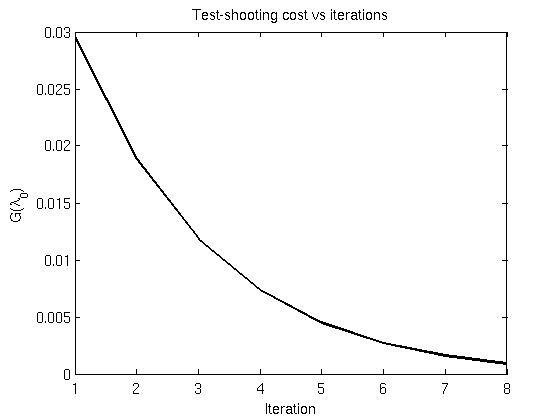
\includegraphics[width=0.8\textwidth]{hw3p3a}
    \end{center}
  \item The optimization condition was $\Vert \mu_\lambda(0) \Vert \le 10^{-3}$.
    \begin{center}
      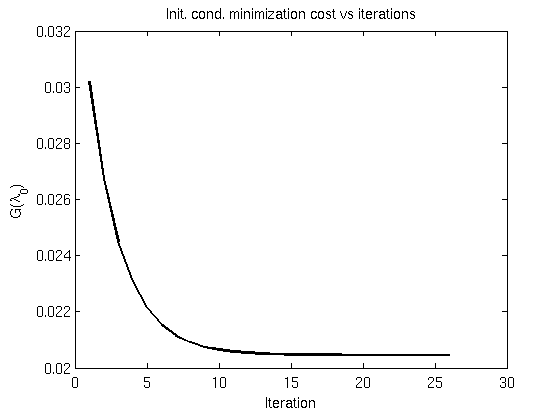
\includegraphics[width=0.8\textwidth]{hw3p3b}
    \end{center}
  \item The test shooting method was both more efficient and more accurate. It achieved a lower final cost and needed less iterations to achieve that cost. I think this is because the test shooting method was created expressly for solving this two-point boundary value problem, while the other algorithm was adapted for this problem. This means the descent direction for the other algorithm is optimal for reducing $\Vert\mu_\lambda(0)\Vert$ and non-optimal for reducing $G(\lambda_0)$. This means that the test shooting method needs less iterations since each descent step results in a greater decrease of the cost.

    Furthremore, the new problem has double the number of dimensions, which could have introduced local minima such that $G(\lambda_0)>0$ when $\Vert\mu_\lambda(0)\Vert=0$. Our choice of $\lambda_0$ could be near one of such local minima. This would explain why the cost for the second algorithm flattens out around $G(\lambda_0)\approx 0.0205$.

    Moreover, from an implementation standpoint, the test shooting method was also easier to implement, because we only need to solve forward in time so we do not need to store the entire trajectories $x(t)$ and $\lambda(t)$. Rather, only the final values $x(T)$ and $\lambda(T)$ are needed. The second algorithm needs the entire $z(t)$ in order to solve backwards for $\mu(t)$.

    \lstinputlisting{hw3p3.m}
  \end{enumerate}

\item I assumed that $T>1$. Notice that in addition to an initial condition, there is also an intermediate condition at $t=1$. Therefore, the costate could have a discontinuity at $t=1$. The optimality conditions are
  \begin{align}
    H &= \frac12 (x^2 + u^2) + \lambda u \\
    \pder{H}{u} &= u + \lambda = 0 \\
    u &= -\lambda \\
    \dot\lambda &= -\pder{H}{x} = -x \\
    \lambda(T) &= \pder{H}{x} = 0
  \end{align}
  Taking the second derivative of $x(t)$ results in
  \begin{gather}
    \ddot x = \dot u = -\dot\lambda = x.
  \end{gather}
  The characteristic equation $z^2 - 1 = 0$ has roots of $\pm 1$, so the optimal $x(t)$ has the form
  \begin{gather}
    x(t) = c_1 e^t + c_2 e^{-t}.
  \end{gather}
  Since $\dot x = u$,
  \begin{gather}
    u(t) = c_1 e^T - c_2 e^{-t}.
  \end{gather}
  For $t\in[0,1]$, the boundary conditions are
  \begin{align}
    x(0) &= c_1 + c_2 = 1 \\
    x(1) &= c_1 e + c_2 e^{-1} = 1
  \end{align}
  Substituting $c_2=1-c_1$ from the first equation into the second,
  \begin{gather}
    c_1 e + (1-c_1)e^{-1} = 1 \\
    c_1 (e - e^{-1}) = 1 - e^{-1} \\
    c_1 = \frac{1-e^{-1}}{e - e^{-1}} \\
    c_2 = \frac{e - 1}{e - e^{-1}} \\
    u(t) = \frac{1-e^{-1}}{e - e^{-1}} e^t - \frac{e - 1}{e - e^{-1}} e^{-t}, \quad 0\le t\le 1
  \end{gather}
  For $t\in[1,T]$, the boundary conditions are
  \begin{align}
    x(1) &= c_1 e + c_2 e^{-1} = 1 \\
    \lambda(T) &= -u(T) = -\dot x(T) = -c_1 e^T + c_2 e^{-T} = 0
  \end{align}
  Equating $c_2$ from the two equations results in
  \begin{gather}
    e - c_1 e^2 = c_2 = c_1 e^{2T} \\
    c_1 = \frac{e}{e^{2T} + e^2} \\
    c_2 = e - \frac{e}{e^{2T} + e^2} e^2 = \frac{e^{2T+1}}{e^{2T} + e^2} \\
    u(t) = \frac{e}{e^{2T} + e^2} e^t - \frac{e^{2T+1}}{e^{2T} + e^2} e^{-t}, \quad t>1
  \end{gather}
  Thus, the optimal control is
  \begin{gather}
    \boxed{u^* = \begin{dcases}
        \frac{1-e^{-1}}{e - e^{-1}} e^t - \frac{e - 1}{e - e^{-1}} e^{-t}, & 0\le t < 1 \\
        \frac{e}{e^{2T} + e^2} e^t - \frac{e^{2T+1}}{e^{2T} + e^2} e^{-t}, & 1\le t\le T
      \end{dcases}}
  \end{gather}

\item \begin{enumerate}
  \item The augmented cost is
    \begin{gather}
      \tilde J(p) = \int_0^T [L + \lambda\trans(f-\dot x)] \dif t = \int_0^T [H - \lambda\trans \dot x] \dif t
    \end{gather}
    A variation $p\mapsto p + \varepsilon$ results in $x\mapsto x+\varepsilon\eta$, where $\eta(0)=0$ since $x(0)$ is fixed. Thus,
    \begin{align}
      \tilde J(p+\varepsilon) &= \int_0^T [H(x+\varepsilon\eta,p+\varepsilon) - \lambda\trans (\dot x + \varepsilon\dot\eta)] \dif t \\
                              &= \int_0^T \left[H + \varepsilon\pder{H}{x}\eta + \varepsilon\pder{H}{p} - \lambda\trans (\dot x + \varepsilon\dot\eta)\right] \dif t + o(\varepsilon) \\
      \tilde J(p+\varepsilon) - \tilde J(p) &= \int_0^T \left[ \varepsilon\pder{H}{x}\eta + \varepsilon\pder{H}{p} - \lambda\trans \dot\eta \right] \dif t + o(\varepsilon) \\
      \intertext{Taking the derivative with respect to $p$ and using integration by parts,}
      \pder{\tilde J(p)}{p} &= \lim_{\varepsilon\to0} \frac{\tilde J(p+\varepsilon) - \tilde J(p)}{\varepsilon} \\
                              &= \int_0^T \left[ \pder{H}{x}\eta + \pder{H}{p} - \lambda\trans \dot\eta \right] \dif t \\
                              &= \int_0^T \left[ \pder{H}{x}\eta + \pder{H}{p} + \dot\lambda\trans \eta \right] \dif t + \lambda\trans(0) \underbrace{\eta(0)}_{=0} - \lambda\trans(T)\eta(T) \\
                              &= \int_0^T \left[ \pder{H}{x} + \dot\lambda\trans \right] \eta \dif t + \int_0^T \pder{H}{p} \dif t - \lambda\trans(T)\eta(T) = 0 \\
      \intertext{Thus, the optimality conditions are}
      \pder{H}{p} &= \pder{f}{p} \lambda = 0 \\
      \dot \lambda &= -\pder{H\trans}{x} = -\pder{L\trans}{x} - \pder{f}{x}\lambda \\
      \lambda(T) &= 0
    \end{align}
  \item We can write the second term of $\partial\tilde J(p)/\partial p$ as
    \begin{gather}
      \mu(T) = \int_0^T \pder{H}{p} \dif t = 0.
    \end{gather}
    since we want the term to be zero. Additionally, taking its derivative
    \begin{gather}
      \dot\mu = \pder{H}{p} = \pder{f}{p} \lambda.
    \end{gather}
    Thus, the optimality conditions can be rewritten as
    \begin{align}
      \dot\lambda &= -\pder{L\trans}{x} - \pder{f}{x}\lambda \\
      \dot\mu &= \pder{f}{p} \lambda \\
      \lambda(T) &= 0 \\
      \mu(T) &= 0
    \end{align}
  \end{enumerate}

\item This is important observation for two reasons:
  \begin{enumerate}[label=\arabic*)]
  \item The costate is dependent on the current state so we do not have to seperately solve the costate equation backwards from time $T$. In fact, using $u^*=-R^{-1}B\trans\lambda$ (shown on midterm), the optimal control is only a function of the state and we don't need to find the costate. This is very advantageous if $T$ is large or infinite. This also avoids having to resort to numerics to find the optimal solution.
  \item Since the optimal control only depends on the current state, this control is optimal for any initial boundary condition on $x(0)$. Additionally, the control still functions if the state changes for some reason, e.g.\ from noise, due to this feedback.
  \end{enumerate}

\end{enumerate}

\end{document}
